\documentclass[a4paper,11pt]{article}

\usepackage[a4paper,margin=2.3cm]{geometry}
\usepackage{graphicx}
\usepackage{cleveref}

\title{Profiling Tools}
\author{Ruairidh MacGregor}
\date{}

\begin{document}

\maketitle

\section{Linux Perf Tools}

Overall this will be only of use on Intel architectures as it is more well supported and provides a significant more amount of hardware performance counters than what it does with AMD. For example it doesn't allow access to specific AMD hardware counters. Output from profiling is not the most clear and can be hard to interpret. The output itself will have to be processed in a script most likely. The following counters will be of use for this study as they target remote/local accesses and output is shown in \Cref{fig:perf_counters}, \Cref{fig:perf_local} \& \Cref{fig:perf_remote}. The general "mem" profiler tool in Linux perf tools captures the above counters profiles all memory accesses, e.g. cache, dram etc. Example output from the "mem" profiler is shown in \Cref{fig:perf_mem} . The major flaw with using these hardware counters is that they lack the specific knowledge from where memory access is coming from, e.g. it doesn't know a thread on node 0 is performing the remote access at node 1, only that a remote access is occuring.

\begin{description}
\item \textbf{Local Access Counters}:
\begin{itemize}
    \item mem\_load\_uops\_llc\_miss\_retired.local\_dram: Data from local DRAM either Snoop not needed or Snoop Miss (RspI)
    \item offcore\_response.demand\_code\_rd.llc\_miss.local\_dram: Counts all demand code reads that miss the LLC and the data returned from local dram
    \item offcore\_response.demand\_data\_rd.llc\_miss.local\_dram: Counts demand data reads that miss the LLC and the data returned from local dram
    \item offcore\_response.all\_demand\_mlc\_pref\_reads.llc\_miss.local\_dram: Counts all local dram accesses for all demand and L2 prefetches. LLC prefetches are excluded
    \item offcore\_response.pf\_l2\_data\_rd.llc\_miss.local\_dram: Counts prefetch (that bring data to L2) data reads that miss the LLC and the data returned from local dram
\end{itemize}
\item \textbf{Remote Access Counters}: 
\begin{itemize}
    \item mem\_load\_uops\_llc\_miss\_retired.remote\_dram: Data from remote DRAM either Snoop not needed or Snoop Miss (RspI)
    \item offcore\_response.demand\_code\_rd.llc\_miss.remote\_dram: Counts all demand code reads that miss the LLC and the data returned from remote dram
    \item offcore\_response.pf\_l2\_data\_rd.llc\_miss.remote\_dram: Counts prefetch (that bring data to L2) data reads that miss the LLC and the data returned from remote dram
    \item offcore\_response.demand\_data\_rd.llc\_miss.remote\_dram: Counts demand data reads that miss the LLC and the data returned from remote dram
    \item offcore\_response.all\_demand\_mlc\_pref\_reads.llc\_miss.remote\_hitm\_hit\_forward: This event counts all remote cache-to-cache transfers (includes HITM and HIT-Forward) for all demand and L2 prefetches. LLC prefetches are excluded
\end{itemize}
\end{description}


\begin{figure}[!htb]
    \centering
    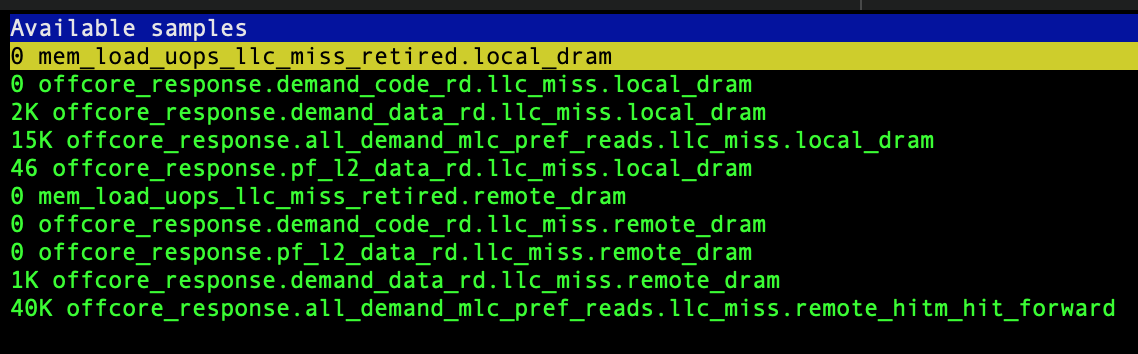
\includegraphics[width=\linewidth]{TechMemo/allocation/images/perf1.png}
    \caption{Output from perf tools using the aforementioned hardware counters. Each line shows the value obtained along with the counter itself. Uses the "SumEuler" benchmark for range 25000. Detailed output for offcore\_response.demand\_data\_rd.llc\_miss.local\_dram is shown in \Cref{fig:perf_local} and for offcore\_response.demand\_data\_rd.llc\_miss.remote\_dram is shown in \Cref{fig:perf_remote}}
    \label{fig:perf_counters}
\end{figure}

\begin{figure}[!htb]
    \centering
    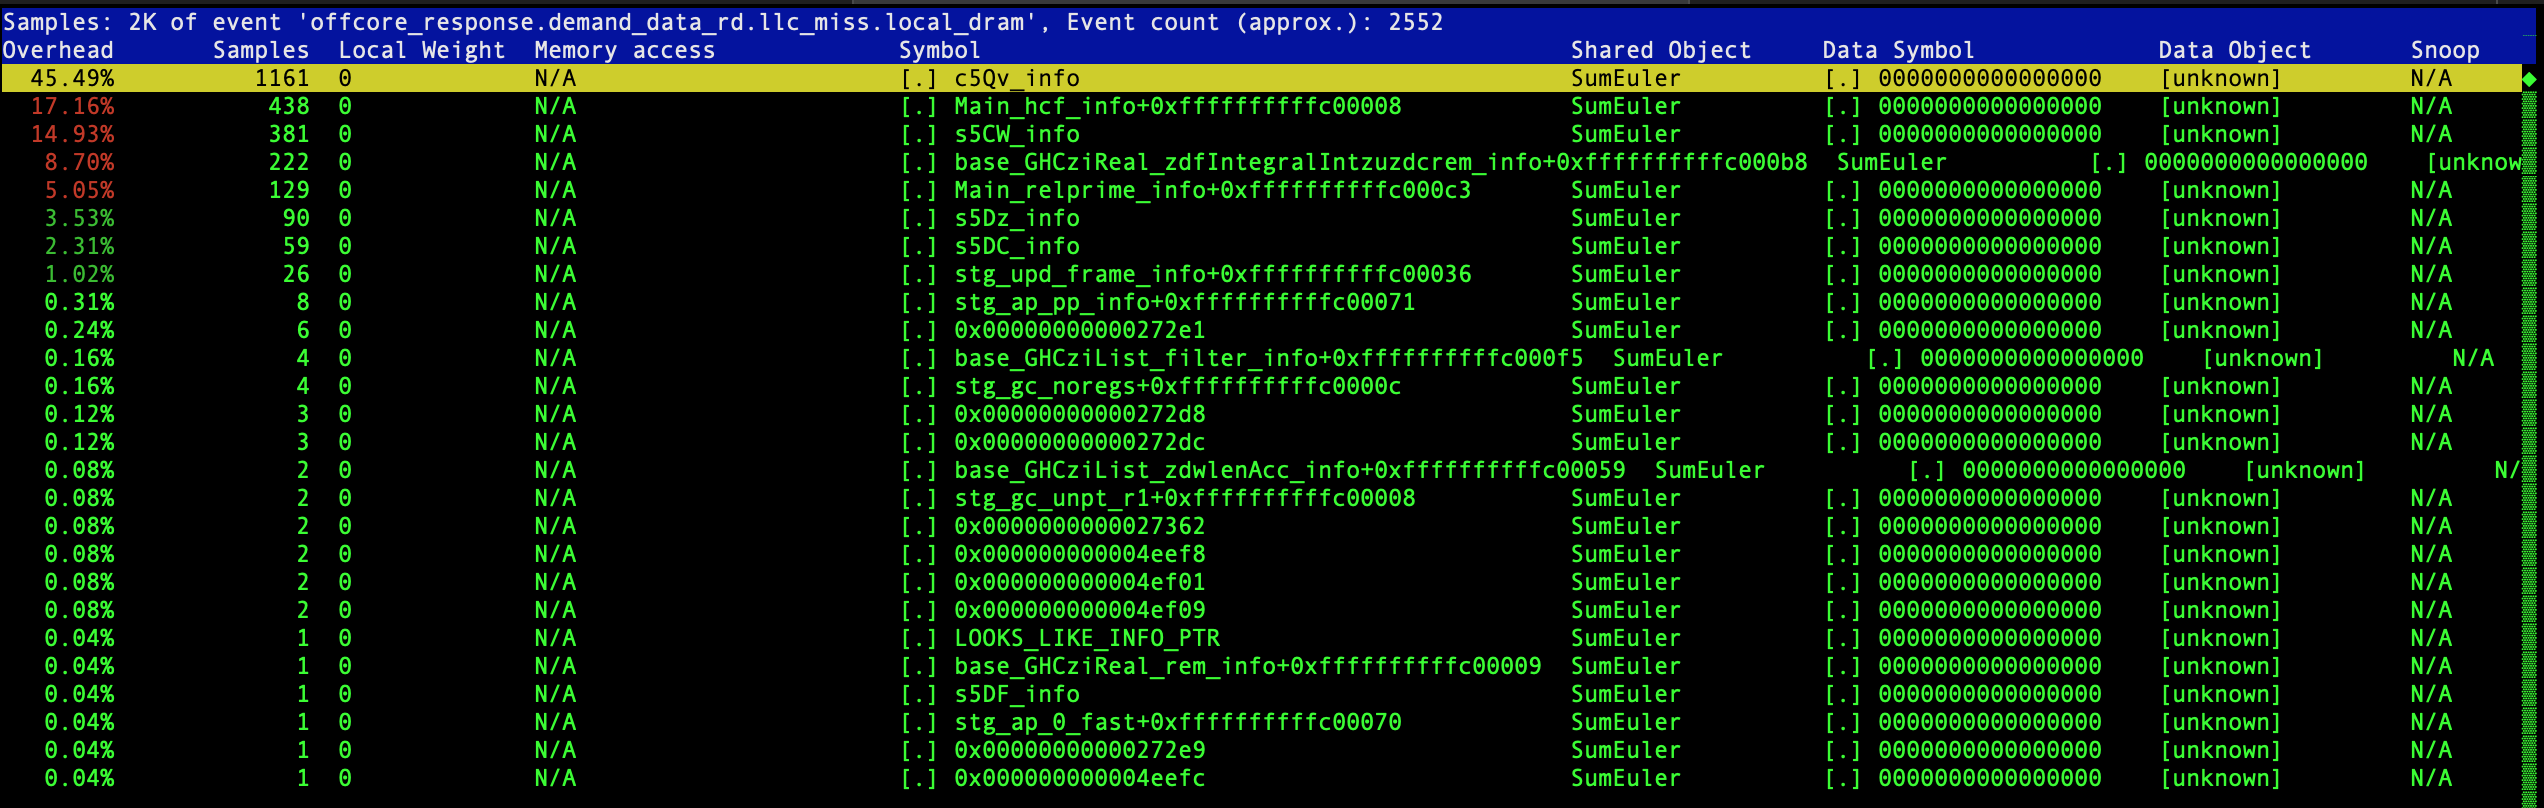
\includegraphics[width=\linewidth]{TechMemo/allocation/images/perf_local.png}
    \caption{Output from offcore\_response.demand\_data\_rd.llc\_miss.local\_dram.}
    \label{fig:perf_local}
\end{figure}

\begin{figure}[!htb]
    \centering
    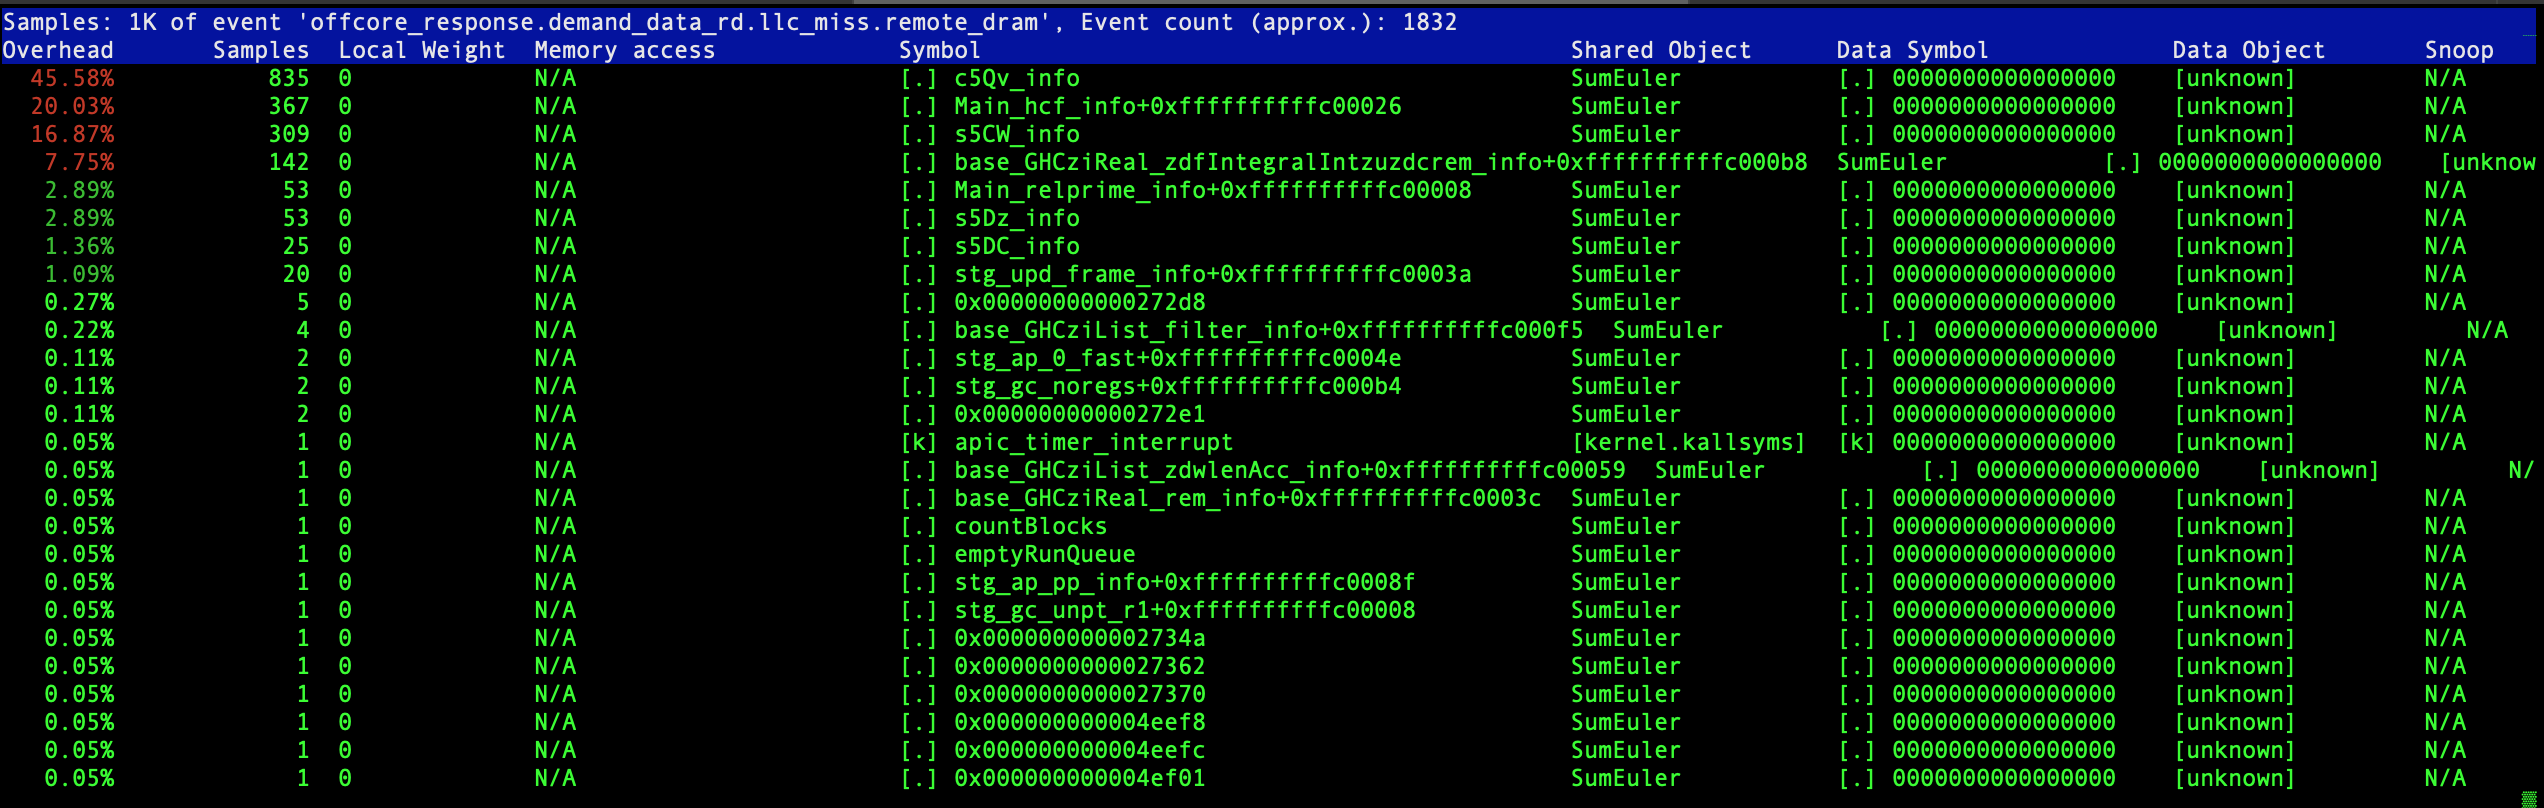
\includegraphics[width=\linewidth]{TechMemo/allocation/images/perf_remote.png}
    \caption{Output from offcore\_response.demand\_data\_rd.llc\_miss.remote\_dram.}
    \label{fig:perf_remote}
\end{figure}


\begin{figure}[!htb]
    \centering
    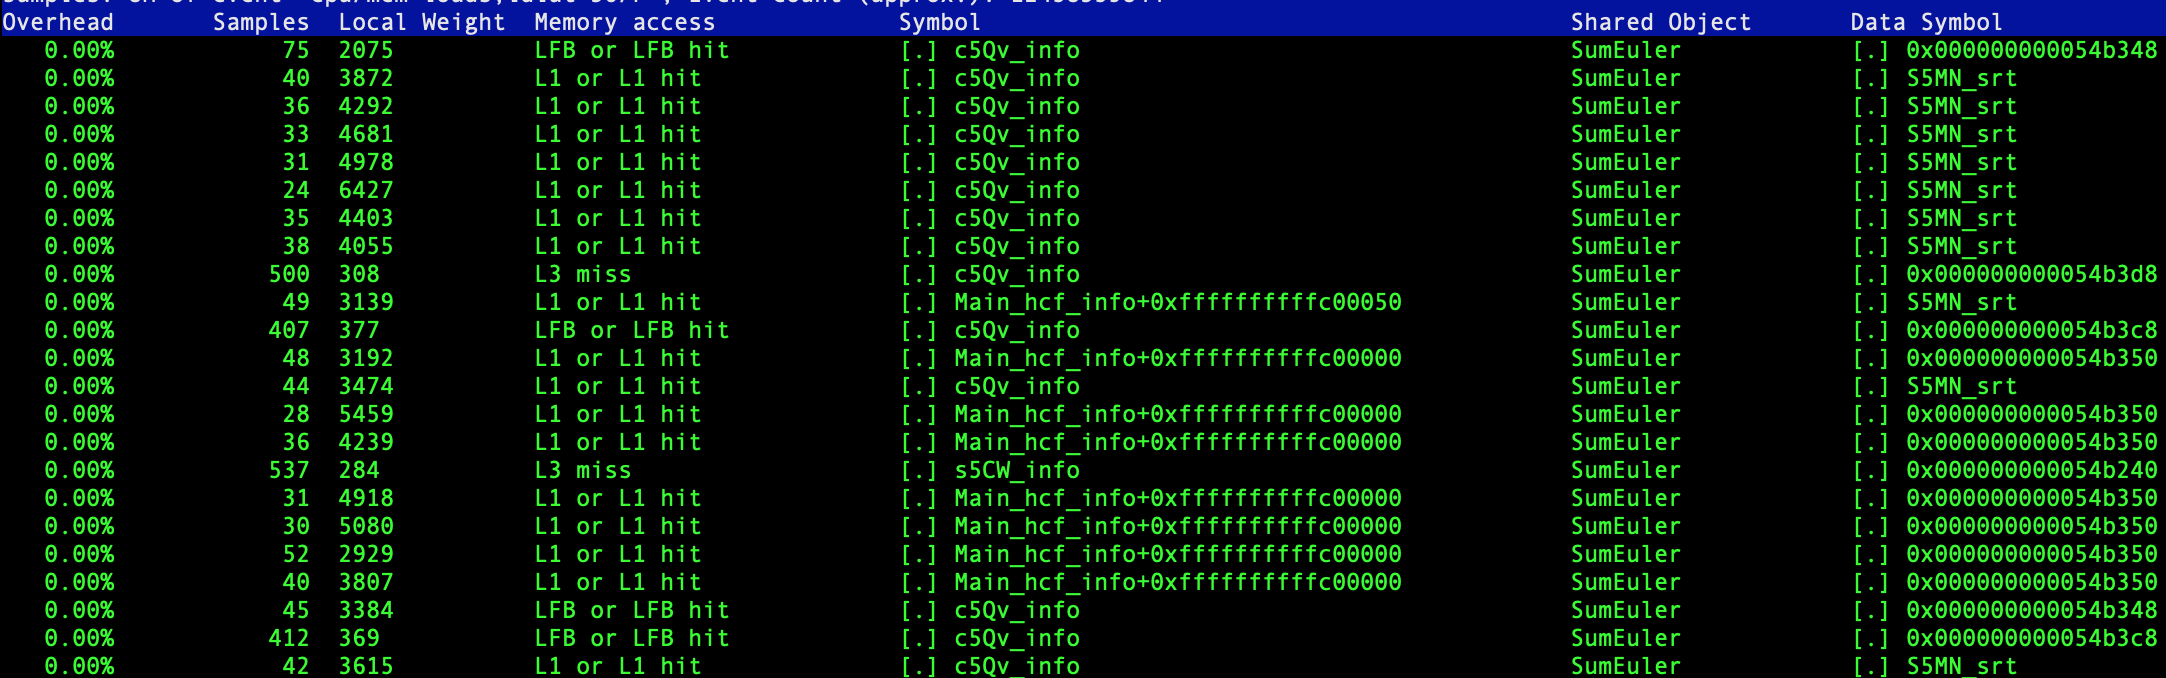
\includegraphics[width=\linewidth]{TechMemo/allocation/images/perf2.png}
    \caption{Output from the perf-mem tool. Showing types of memory access. The difficulty from using solely this tool is that it doesn't indicate where the L3 miss was satisfied from, e.g. if it was remote or local. Hence the need for the specific afore-mentioned counters.}
    \label{fig:perf_mem}
\end{figure}


\section{GHC Profiling}

The GHC memory profiler will be of use for recording mean/peak allocation rate. It presents the most detailed information found and produces an output graph as a result, depicting how the allocation rate varies as the program executes. \Cref{fig:alloc_prsa} and \Cref{fig:alloc_parfib} shows output allocation rate graphs from GHC. The GHC profiler also provides garbage collection metrics which lack the specific NUMA requirements for this work. Extensions to this tool appear most likely as the garbage collector is specific to GHC and therefore an existing tool is highly unlikely to be discovered. \Cref{fig:gc_prof}
shows output from the garbage collector profiler. There is another memory related profiler

\begin{figure}[!htb]
    \centering
    \includegraphics[width=\linewidth]{Interim Report/images/prsa.png}
    \caption{An example mean/peak allocation rate graph obtained from the existing GHC memory profiler run on the parallel RSA encryption algorithm from the nofib benchmark suite. The graph is broken down by closure type and is outlined on the legend.}
    \label{fig:alloc_prsa}
\end{figure}

\begin{figure}[!htb]
    \centering
    \includegraphics[width=\linewidth]{Interim Report/images/parfib.png}
    \caption{Another mean/peak allocation rate graph produced by the GHC heap profiler, broken down by closure type. The STACK closure appears to be significantly more of a memory burden than others and appears to be more non-deterministic than the others, e.g. the others all increase near enough at their own individual rate and then flatten out, meanwhile STACK varies throughout more and never really flattens out. The maximum difference between the peak allocation from STACK to the next highest appears to be well over ~1800kb.}
    \label{fig:alloc_parfib}
\end{figure}

\begin{figure}[!htb]
    \centering
    \includegraphics[width=\linewidth]{Interim Report/images/gc_prof.png}
    \caption{Existing garbage collector profiler in GHC. Showing the garbage collection total runtimes, also per generation, pause times, frequency (e.g. collections) and collections in parallel (e.g. par collections). Other data such as data copied between different generations is also shown. As discussed, the tool currently lacks specific NUMA information relating to regions.}
    \label{fig:gc_prof}
\end{figure}

\begin{figure}[!htb]
    \centering
    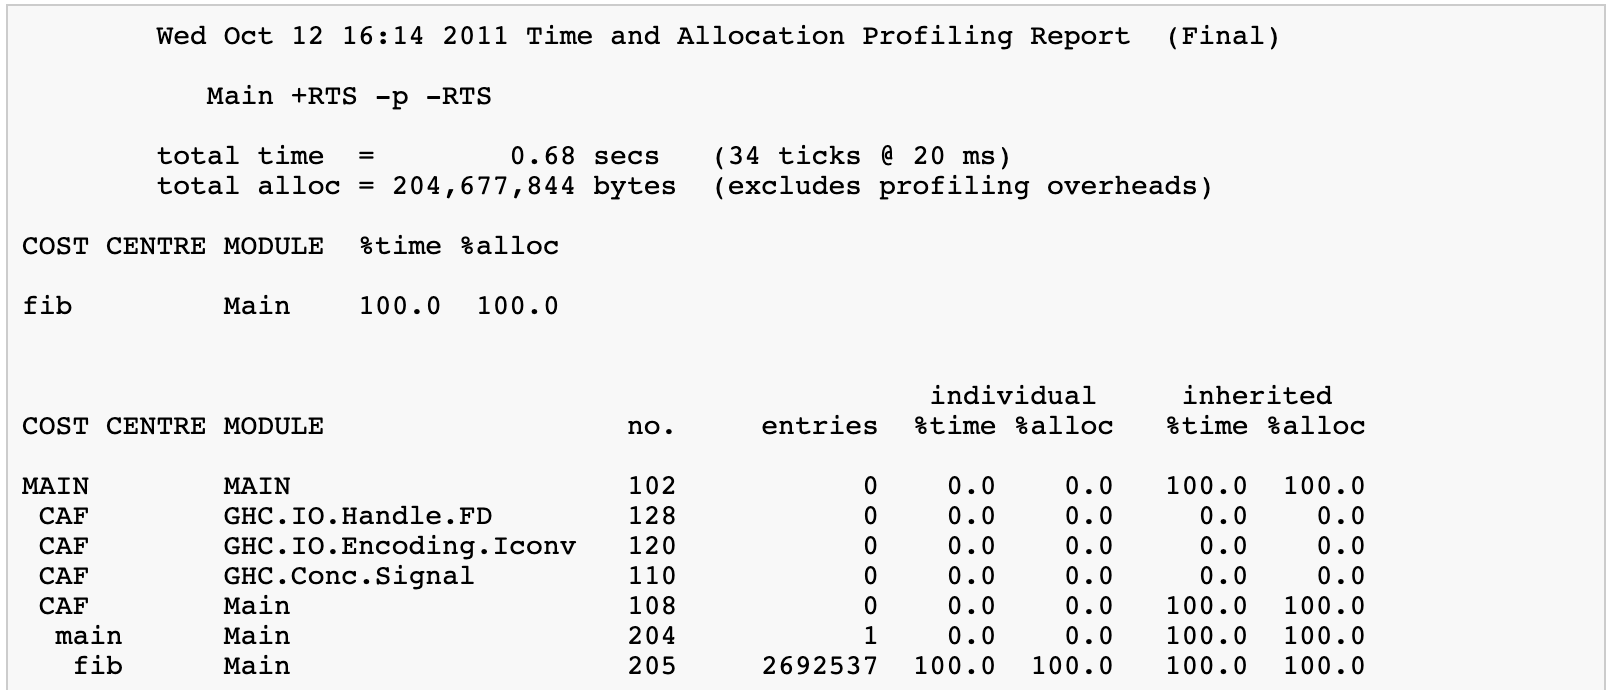
\includegraphics[width=\linewidth]{TechMemo/allocation/images/ghc_mem.png}
    \caption{Other memory profiler in GHC. Shows breakdowns of memory consumption by functions in the Haskell code. Overall, not useful for this study.}
    \label{fig:ghc_mem}
\end{figure}

\section{Numaprof}

Numaprof appears to be the most detailed profiler that has been used and is also platform independent and doesn't rely on hardware counters. It provides detailed access patterns, shown in the access matrices in \Cref{fig:access_matrix} \& \Cref{fig:access}. Major downside is that it doesn't track specific unpinned accesses, e.g. thread running on node 0 accessing node 1, it just tracks it as unpinned access to region 1 - little bit more informative than hardware counters but needs either (A) extended or (B) find another tool.

\begin{figure}[!htb]
    \centering
    \includegraphics[width=0.5\linewidth]{Interim Report/images/accessMatrix.png}
    \caption{An example access matrix produced as output from the numaprof tool on the "Blackscholes" benchmark from the nofib suite. An entry (i,j) in the matrix means NUMA region $i$ accessing memory in region $j$ ($0 \leq i,j < N$, $N$ is the total number of NUMA regions available). The bottom row shows accesses from unpinned threads to remote regions, following the same format for a normal entry, e.g. unpinned thread in NUMA region 0 accessing NUMA region 1. Note, one needs to "hover" the cursor over an entry to get the number of accesses. The more apparent the shade of red is in an entry indicates significantly more accesses, relative to another region with a darker colour, e.g. blue.}
    \label{fig:access_matrix}
\end{figure}

\begin{figure}[!htb]
    \centering
    \includegraphics[width=0.5\linewidth]{Interim Report/images/acc.png}
    \caption{Access matrix produced from the SumEuler benchmark from the nofib suite using the numaprof tool. Computes Euler totient range from 0 to 200000 with a chunk size of 250. Results show some strong locality of reference with the darker colours going from the diagonal from entry (0,0) to (7,7). However, there appears to be an imbalance in which all regions access region 7 significantly higher than others, indicated by the bright red colours. This is a memory intensive benchmark with a large input.}
    \label{fig:access}
\end{figure}

\begin{figure}[!htb]
    \centering
    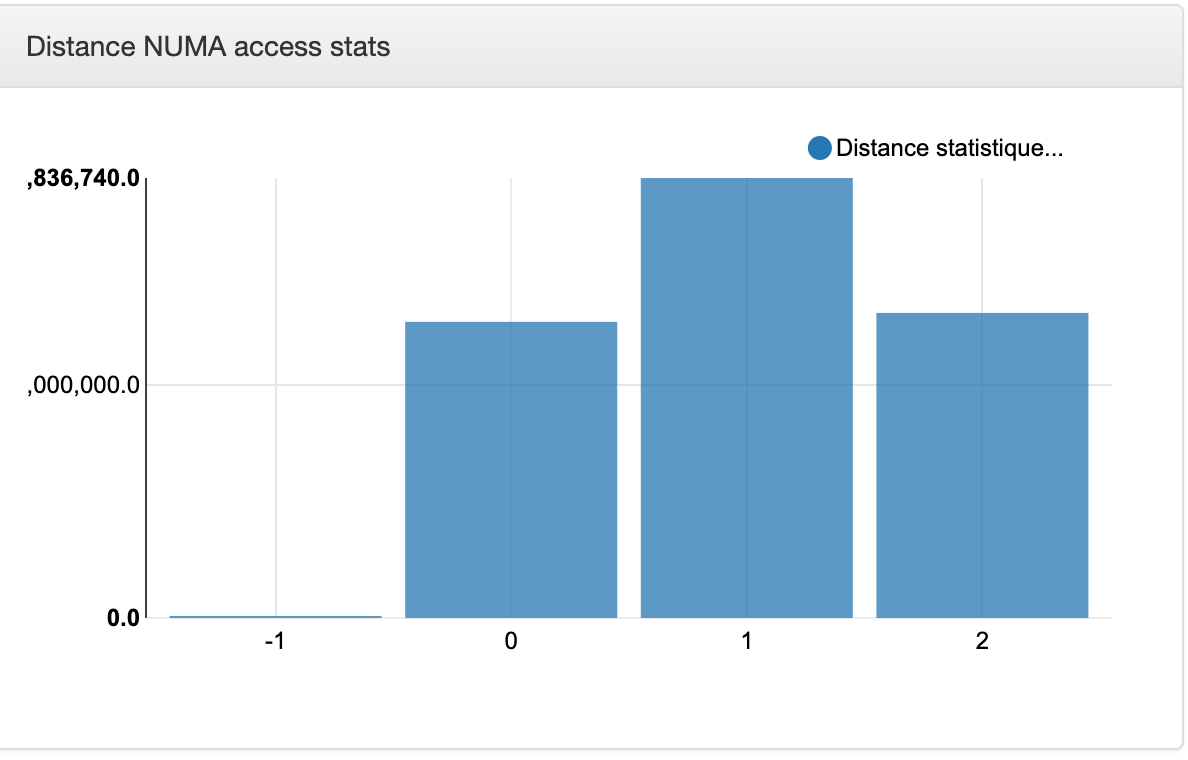
\includegraphics[width=\linewidth,height=0.6\linewidth]{TechMemo/allocation/images/numaprof_dist.png}
    \caption{NUMA distance statistics. This is dependent on the total number of distinct distances between nodes in the architecture. The output of the command "numactl --hardware" will give these distinctions. For example on Togian, there is 3 distinct distances, 10, 16 and 22. NUMA distance 0 means accessing the same node and corresponds to 10, 1 corresponds to 16 and 2 corresponds to 22. The numbers 10, 16 and 22 are relative distances but closely resemble the access latency.}
    \label{fig:numa_dist}
\end{figure}

\begin{figure}[!htb]
    \centering
    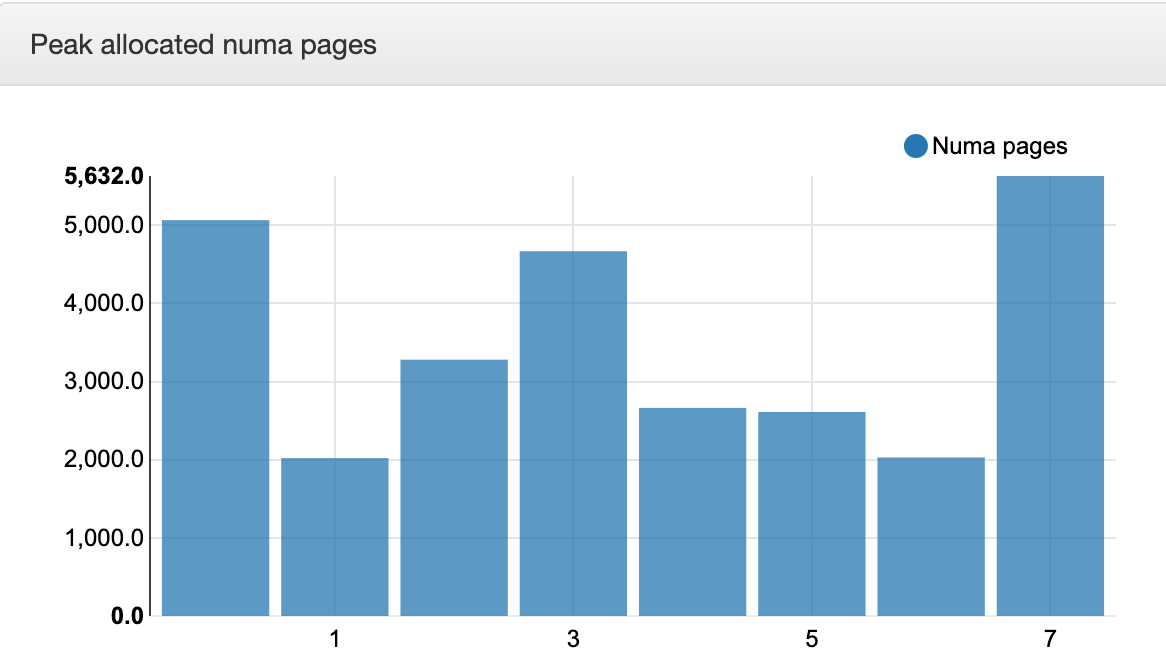
\includegraphics[width=\linewidth]{TechMemo/allocation/images/numaprof_peak.png}
    \caption{Peak allocated NUMA pages per region. Each bar corresponds to a region and the height of the bar indicates the number of pages allocated on said region. Note: this was run on SumEuler with 25000 range.}
    \label{fig:numa_peak}
\end{figure}

\section{Intel VTune}

This is very similar to Perf tools (as perf uses the same counters). However, this is much more informative and clear what each entity means. Documentation is excellent, both user guide and on the client, e.g. you can hover over boxes and a description of what something means appears. Also, very easy to export data to CSVs etc. Only difficulty is the hardware counters must be used on Intel and won't suffice on AMD. I believe the software events can be used, but anything lower than that is specific to Intel. This tool has been able to record information that I haven't been able to do so on perf tools, these include access latency (\Cref{fig:latency}) and bandwidth utilization (\Cref{fig:bandwidth}).

\begin{figure}[!htb]
    \centering
    \includegraphics[width=\linewidth]{Interim Report/images/latency.png}
    \caption{Latency histogram produced by the Intel VTune profiler and using the "Blackscholes" application from the nofib benchmark suite. This can be broken down further in Intel VTune, but this is the general idea of what will be produced as a deliverable. A general observation of this is that most load instructions have low latency (latency measured in clock cycles).}
    \label{fig:latency}
\end{figure}

\begin{figure}[!htb]
    \centering
    \includegraphics[width=\linewidth]{Interim Report/images/band.png}
    \caption{Bandwidth utilization histogram produced by the Intel VTune profiling tool using the "Blackscholes" application from the nofib benchmark suite. A general observation of this is that all objects don't utilize the bandwidth a great deal. This is the same application run in \Cref{fig:latency}, which shows the latency per load instruction was in general very low, therefore the bandwidth utilization also being very low contibutes to this as there is reduced contention. Note: the "Low, Medium, High" bar located at the bottom of the graph is user definable - those are just the default.}
    \label{fig:bandwidth}
\end{figure}

\section{AMD uProf}

This tool is supposed to be the AMD equivalent of VTune and does provide a lot of low level hardware counter access. However, those counters that are of interest have not successfully been recorded - I have a strong suspicion that this is to do with the AMD processor available not being supporting the specific hardware counters required as it produces an error whenever I try to use it on Togian. Specifically: "Error: (null)". The counters tried were:

\begin{description}
\item PMCx1E0: CPU to DRAM Requests to Target Node
\item PMCx1E2: CPU Read Command Latency to Target Node 0-3
\item PMCx1E3: CPU Read Command Requests to Target Node 0-3
\item PMCx1E4: CPU Read Command Latency to Target Node 4-7
\item PMCx1E5: CPU Read Command Requests to Target Node 4-7
\item PMCx1E6: CPU Command Latency to Target Node 0-3/4-7
\item PMCx1E7: CPU Requests to Target Node 0-3/4-7
\end{description}

\section{Numastat}

Provides access to per region local access and remote accesses, however lacks sufficient information with regards to where accesses are coming from as uses hardware counters. Runs on both Intel and AMD. 

\section{PAPI}

Cross platform tool that provides access to hardware counters in source code. Obviously only AMD hardware counters can be accessed on AMD devices etc. 


\section{Other Profiling Tools}

The following tools have not been experimented but appear to be inadequate for this work, based on documentation from research papers or online posts etc. Therefore is only as useful as what the hardware provides and doesn't record any specific events itself within the library.

\begin{description}
\item \textbf{NUMATOP}: Counts the number of local and remote accesses of all running applications and displays the result into the terminal. The tool relies on hardware counters to determine this. Like with other hardware counter focused tools, it doesn't provide information on where the memory accesses are coming from. Only supported on Intel Xeon processors: 5500-series, 6500/7500-series, 5600 series, E7-x8xx-series, and E5-16xx/24xx/26xx/46xx-series.
\item \textbf{SNPERF}: provides charts with memory accesses on each NUMA domain over time with a given process. It relies on hardware counters of the Origin 2000 architecture. This is useful for checking if memory bandwidth is balanced across nodes. Tool currently is not available and was only available on an unusual architecture.
\item \textbf{Memphis}: is a tool making deep instrumentation on AMD Opteron hardware counters. It uses event sampling to report the domain access count onto source code lines. However, tool is not available anymore.
\item \textbf{MemProf}: focuses on access patterns specific for NUMA. The tool tracks each thread memory access flow by using a kernel module and tracking threads binding to detect specific bad access patterns. Relies on Instruction Based Sampling from AMD.
\item \textbf{NUMAgrind}: The tool is based on architecture simulation, so not relying on hardware counters. It simulates all the cache details and page affinity.
\item \textbf{HPCToolkit}: It uses hardware counters and sampling to track the information. It provides all the usage information of a variable in one go: allocation
site, first touch site and all access site. It also provides a summary of the access
pattern over threads so the developer can look at how the memory accesses are
distributed and might find some reordering or packing to improve data locality. However, the NUMA part of this tool is not publicly available.
\end{description}

\section{REMEMBER VAMPIR PROFILING}

\end{document}
